\documentclass{article}
\usepackage{graphicx}
\usepackage{multicol} % use to multiple column in itemize
\usepackage{float}
\usepackage{setspace}
\setlength{\parskip}{0.5em}

\begin{document}

\title{Bias Variance Trade-Off}
\author{Cong Cuong PHAM}

\maketitle

\begin{abstract}
This document introduces the trade-off between bias and variance.
\end{abstract}

\section{Introduction}
\subsection{Bias Variance trade-off}
\begin{itemize}
	\item The bias-variance trade-off is the point where we are adding just noise by adding model complexity (flexibility).
	\item The {\bf{training error}} goes down as it has to, but the {\bf{test error}} is starting to go up.
	\item The model after the bias trade-off begins to {\bf{overfit}}.
\end{itemize}

\begin{figure}[H]
\centering
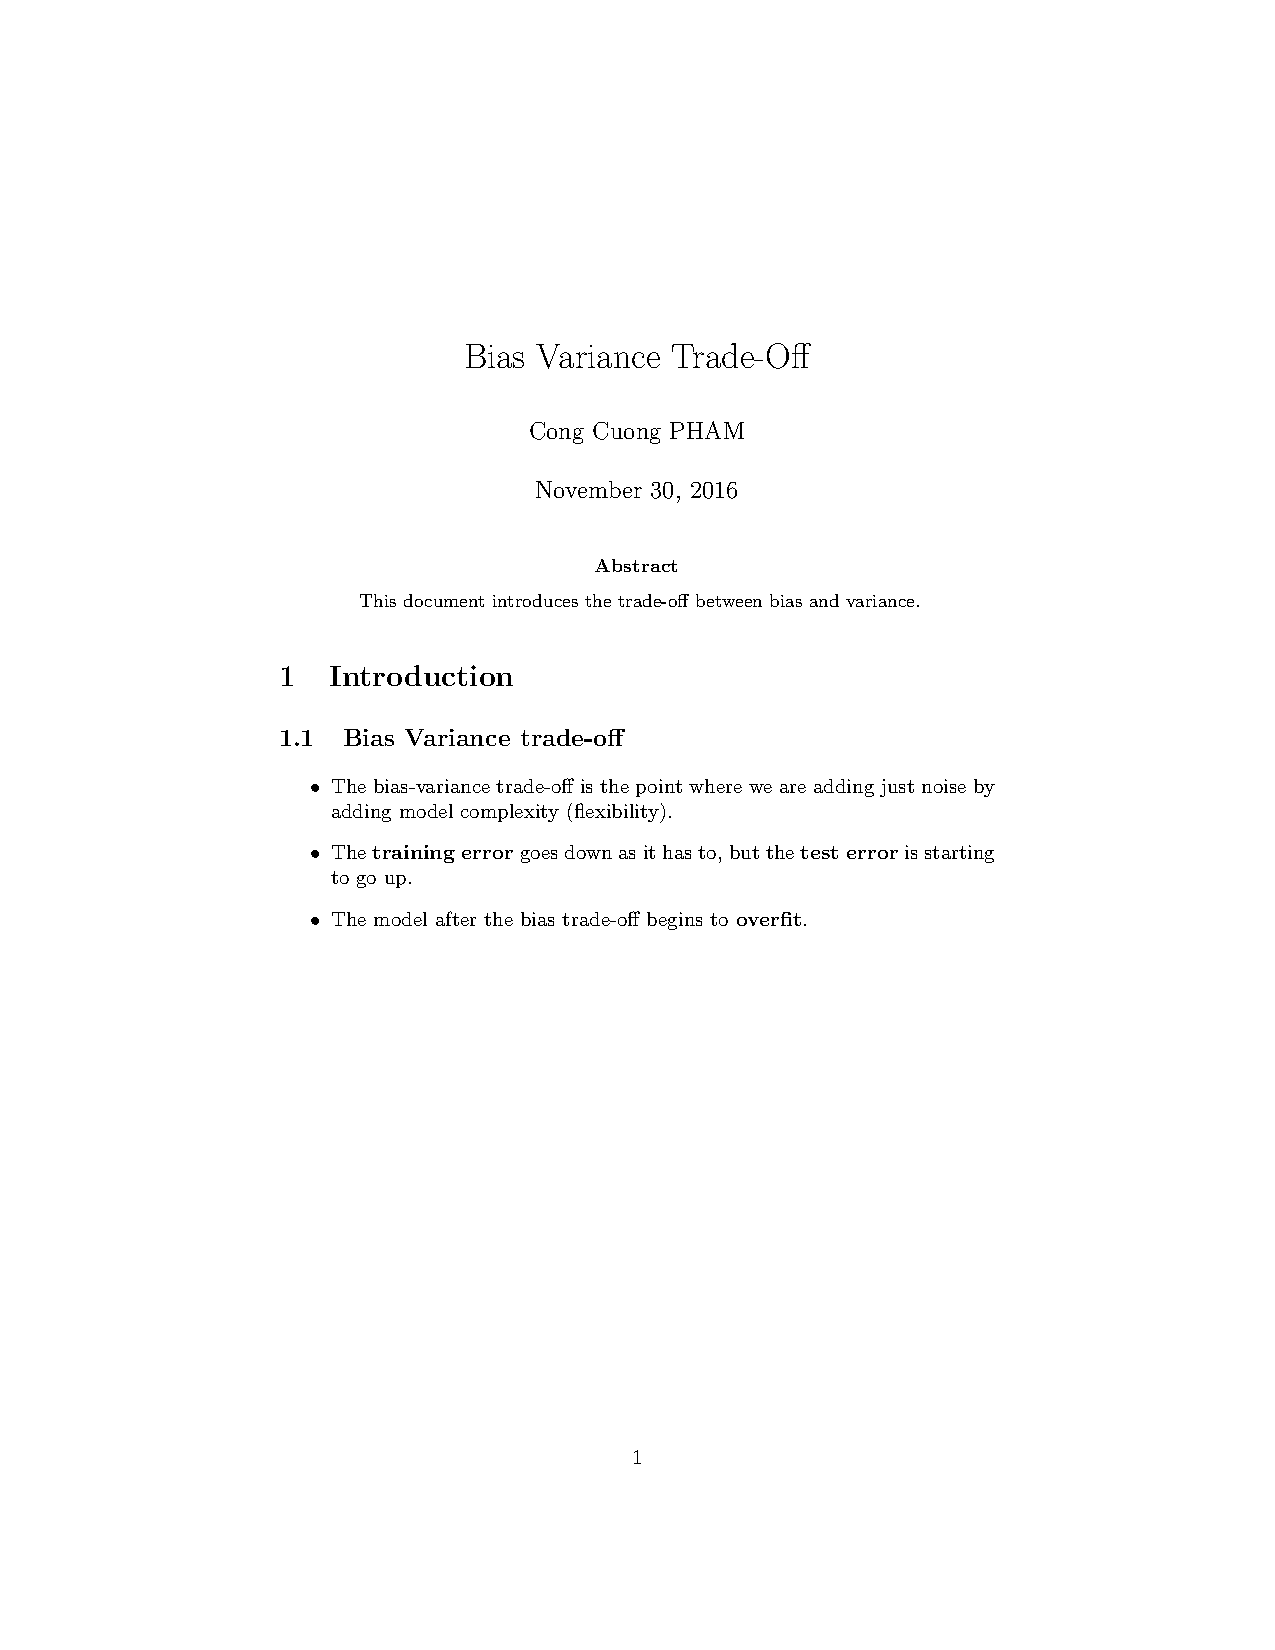
\includegraphics[width=0.6\linewidth]{pic/bias-variance-trade_off.png}
\caption{Bias variance trade-off. The center of the target is a model that perfectly predicts the correct values. As we move away from the bulls-eye, our predictions get worse and worse.}
\end{figure}

\begin{itemize}
	\item A common temptation for beginners is to continually add complexity to a model until it fits the training set very well.
\end{itemize}

\begin{figure}[H]
\centering
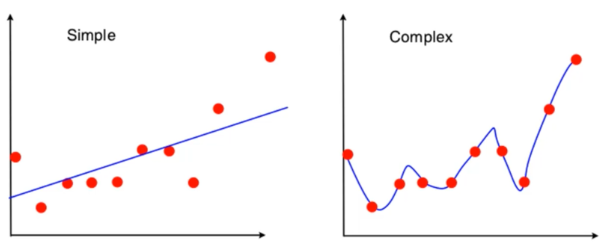
\includegraphics[width=0.9\linewidth]{pic/simple-complex-model.png}
\caption{Use simple-complex model to fit training data. Complex model may overfit to training data and cause large errors on new data, such as the test set.}
\end{figure}

\begin{figure}[H]
\centering
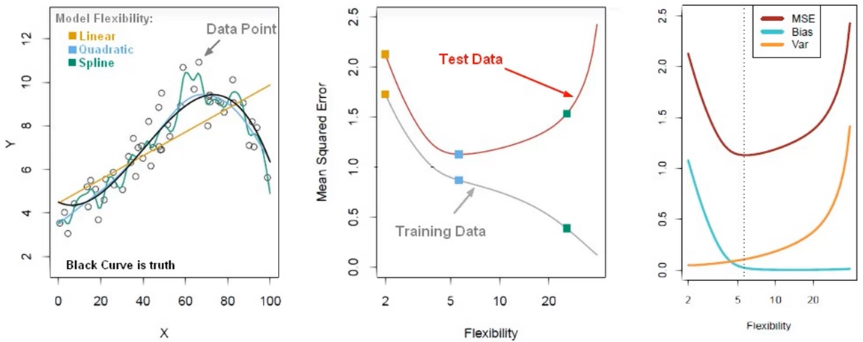
\includegraphics[width=\linewidth]{pic/MSE-complexity-relationship.png}
\caption{The relationship between Mean Squared Error (MSE) and the complexity (flexibility). A black curve with some ``noise'' points off it is used to represent the True shape the data follows.}
\end{figure}

\begin{figure}[H]
\centering
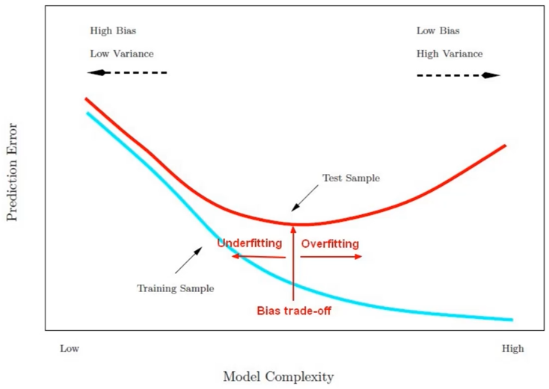
\includegraphics[width=0.8\linewidth]{pic/prediction_error-complexity-relationship.png}
\caption{The relationship between Prediction Error and the complexity (flexibility).}
\end{figure}


\end{document}

